
%!TEX ROOT=ctutest.tex

\chapter{Dynamický model}

Pro výpočet a predikci spotřeby elektrické energie robotického manipulátoru je nezbytné vytvořit matematický model robotu popisující jeho dynamiku.

Robot KUKA KR5 Arc je mechanický systém tvořený šesti sériově spojenými rameny. Každé rameno se může nezávisle na ostatních otáčet otáčet kolem své vlastní osy rotace. Okamžitou konfiguraci ramen robotu i pozici koncového efektoru v prostoru je tak možné popsat šesti souřadnicemi odpovídajícími úhlům natočení jednotlivých os. Jedná tak o systém se šesti stupni volnosti. K popisu jeho dynamiky je proto potřeba celkem 6 rovnic druhého řádu. Celkově se tedy jedná o dynamický systém dvanáctého řádu. 

\section{Pohybové rovnice}
\label{pohybove_rovnice_sec}
K odvození pohybových rovnic je možné použít jeden ze dvou základních přístupů a to Newton-Eulerovu metodu nebo Euler-Lagrangeovu metodu [\cite{rob_mod_control}]. 

Newton-Eulerova metoda je založena na přístupu k systému jako k soustavě jednotlivých jeho součástí a vyžaduje určení pohybových rovnic každé jednotlivé komponenty. Výsledná dynamika je poté součtem dynamik všech dílčích komponent systému. Protože jsou jednotlivé osy sériových robotických manipulátorů vzájemně kinematicky propojeny, jsou i pohybové rovnice jednotlivých jejich os závislé na pohybu ostatních os. 

Euler-Lagrangeova metoda naopak přistupuje k systému jako k celku a je založena na určení Lagrangianu, který je definován jako rozdíl celkové kinetické a potenciální energie systému. Dynamické rovnice systému je poté možné odvodit vypočtením Lagrangeových rovnic druhého druhu pro všechny stupně volnosti systému.

Oba přístupy nakonec vedou ke stejným rovnicím. Protože je pohyb a dynamika systému popisována pomocí úhlů na jednotlivých osách a jejich derivací, vyskytují se v jeho rovnicích nelineární goniometrické členy. Výsledné rovnice systému jsou proto silně nelineární. 

V případě robota KUKA KR5 Arc se jedná o soustavu 6 rovnic o celkem 24 neznámých  - moment síly, poloha, úhlová rychlost a úhlové zrychlení pro každou z šesti os. Pro zlepšení přehlednosti rovnic systému je možné tyto rovnice zapsat v následujícím maticovém tvaru jako 

\begin{equation}
T = M(\dot{\theta},\theta)\ddot{\theta} + C(\dot{\theta},\theta)\dot{\theta} + G(\theta)
\label{dyn_rovnice_eq}
\end{equation}

kde

\begin{description}
\item[$T = {\big[T_1  \dotsm  T_n\big]}^{T}$] je vektor momentů sil působících na jednotlivé osy robota
\item[$\ddot \theta = {\big[\ddot \theta_1  \dotsm  \ddot \theta_n\big]}^{T}$] je vektor úhlových zrychlení na jednotlivých osách
\item[$\dot \theta = {\big[\dot \theta_1  \dotsm  \dot \theta_n\big]}^{T}$] je vektor úhlových rychlostí na jednotlivých osách
\item[$M\big(\dot \theta, \theta\big)$] je matice setrvačnosti tvořena tenzory setrvačnosti jednotlivých os
\item[$C\big(\dot \theta, \theta\big)$] je matice Coriolisových a odstředivých momentů sil působících na jednotlivé osy
\item[$G\big(\theta\big)$] je matice gravitačních sil působících na jednotlivé osy
\item[$n$] je počet os
\end{description}

K výpočtu okamžité spotřeby elektrické energie je nutné řešit inverzní dynamickou úlohu (rovnice \ref{dyn_rovnice_eq}), kdy se z okamžitých poloh, úhlových rychlostí a úhlových zrychlení na jednotlivých osách robota vypočítají točivé momenty, kterými působí motory. 

Moment síly motoru je závislý na proudu protékajícím jeho vinutím. Tuto závislost je obvykle možné aproximovat lineární závislostí [\cite{sbornik}] a psát jako
\begin{equation}
T\big(t\big) = KI\big(t\big)
\label{torque_current_eq}
\end{equation}

kde

\begin{description}
\item[$T\big(t\big) {\big[Nm\big]}$] je moment síly motoru 
\item[$K {\big[Nm/A\big]}$] je momentová konstanta 
\item[$I\big(t\big) {\big[A\big]}$] je proud protékající motorem 
\end{description}

Nástroj TRACE robotu KUKA KR5 Arc tímto způsobem počítá točivé momenty jednotlivých motorů. Momentové konstanty jednotlivých motorů jsou obvykle poskytovány výrobci a je možné je dohledat v jejich dokumentaci. 

\section{Tření}

Odvozené rovnice dynamiky robota popsané výše v sekci \ref{pohybove_rovnice_sec} popisují pouze ideální model, ve kterém nedochází k žádným energetickým ztrátám. V reálných motorech ale kromě elektrických ztrát v jejich vinutích dochází také k energetickým ztrátám v důsledku tření v ložiscích motorů, rotačních os a tření v převodovkách.

Úplný popis tření v rotačních systémech je relativně komplikovaný, protože se jedná o silně nelineární děj, který navíc obecně bývá závislý na čase a na okolních podmínkách. Proto se zpravidla pro modelování tření používá zjednodušený model popisující tření jako kombinaci viskózního a Coulombova tření \cite{fric_eff_analysis}. 

Viskózní tření motoru je moment síly působící proti otáčení motoru, který je lineárně závislý na jeho rychlosti rotace. Při nulové rychlosti je třecí moment síly nulový a s rostoucí rychlostí se zvyšuje. Při změně směru otáčení motoru se mění i směr působení třecího momentu. 

Coulombovo tření je naopak na rychlosti rotace nezávislé. V systému je přítomno vždy a vždy se stejnou magnitudou. Mění se pouze se změnou směru otáčení, kdy mění znaménko.

Tento použitý popis tření je popsán rovnicí 

\begin{equation}
T_f = f_v\dot{\theta} + f_csign(\dot{\theta})
\label{fric_eq}
\end{equation}

kde

\begin{description}
\item[$T_f$] je moment síly generovaný třením 
\item[$f_v$] je koeficient viskózního tření 
\item[$f_c$] je koeficient Coulombova tření 
\end{description}

Na následujícím obrázku (obr. \ref{treni_pic}) je znázorněn použitý model tření včetně jeho jednotlivých složek. Na vodorovné ose je uvedena úhlová rychlost otáčení, na svislé ose je generovaný třecí moment síly.

\newpage
\begin{figure}[ht]
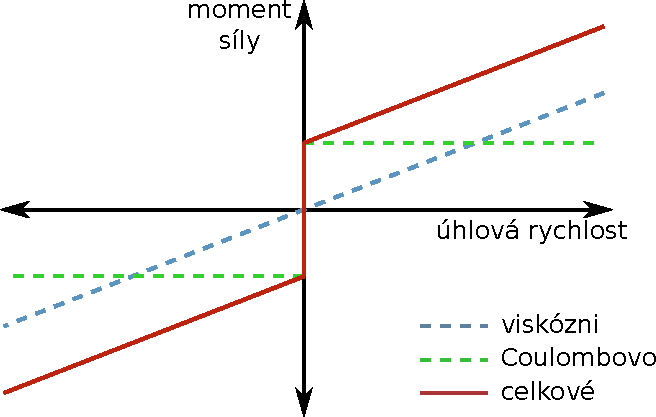
\includegraphics[width=0.65\textwidth]{treni}
\caption{Model tření os}
\label{treni_pic}
\end{figure}

Doplněním rovnic tření \ref{fric_eq} do dynamických rovnic robota \ref{dyn_rovnice_eq} se získají celkové rovnice dynamiky robota ve tvaru

\begin{equation}
T = M(\dot{\theta},\theta)\ddot{\theta} + C(\dot{\theta},\theta)\dot{\theta} + G(\theta) + F_v\dot{\theta} + F_csign(\dot{\theta})
\label{celkova_dyn_rovnice_eq}
\end{equation}

kde

\begin{description}
\item[$F_v = {\big[F_{v1}  \dotsm  F_{vn}\big]}^{T}$] je vektor koeficientů viskózního tření v jednotlivých osách
\item[$F_c = {\big[F_{c1}  \dotsm  F_{cn}\big]}^{T}$] je vektor koeficientů Coulombova tření v jednotlivých osách
\end{description}

\section{Elektrický výkon a spotřeba elektrické energie}
\label{el_vykon_ch}
Výkon je obecně definován jako práce $W$ vykonaná za jednotku času [\cite{zemanek}]. Pro okamžitý výkon platí rovnice

\begin{equation}
p(t) = \frac{dW}{dt}
\end{equation}

Protože se v tomto případě jedná o elektrickou práci, resp. práci elektromagnetického pole, je tato práce definovaná jako element náboje $dq$ přenesený mezi dvěma místy s napětím $u$. Po jejím dosazení platí vztah

\begin{equation}
p(t) = \frac{u(t)dq}{dt}
\end{equation}

Protože element náboje $dq$ přenesený za čas $dt$ odpovídá okamžitému proudu, je možné vzorec pro okamžitý výkon upravit na

\begin{equation}
p(t) = u(t)\frac{dq}{dt} = u(t)i(t)
\end{equation}

Spotřebovaná elektrická energie je definovaná jako celková elektrická práce, která byla vykonaná spotřebičem za čas $t$. Platí pro ni vztah

\begin{equation}
W = Pt
\end{equation}

Pro její okamžitou hodnotu lze tento vzorec upravit následovně

\begin{equation}
w(t) = p(t)\frac{dt}{dt} = p(t)
\end{equation}  

Z tohoto vztahu vyplývá, že okamžitá spotřeba elektrické energie spotřebiče odpovídá jeho elektrickému výkonu. Pro účely modelování spotřeby elektrické energie robotického manipulátoru tedy stačí modelovat robota z hlediska jeho okamžitého elektrického výkonu.  

\subsection{Elektrický výkon robotu}

Celkový elektrický výkon robotického manipulátoru je závislý na elektrickém výkonu jednotlivých jeho součástí. Elektrická část robotu je tvořena pohony ramen robotu, senzory poloh, teplot a dalších veličin a jeho centrální řídicí jednotkou. 

Je možné předpokládat, že spotřebovaný výkon jednotlivých senzorů a hlavní řídicí jednotky bude přibližně konstantní, protože musí pracovat stejně ze všech podmínek. Tato složka výkonu $P_s$ bude přispívat k celkovému výkonu robotického systému, nebude ale závislá na jeho dynamice. Celkový výkon robotu bude tedy tvořen touto stálou složkou $P_s$ a elektrickým výkonem pohonů robotu.

Osy robotu jsou poháněny elektrickými synchronními servomotory s permanentními magnety. K výpočtu výkonu elektrických motorů je potřeba vytvořit model jejich vinutí. Přestože se jedná o třífázové motory, nejsou k dispozici informace o průbězích napětí a proudu na jednotlivých fázích. Řídicí systém robotu KUKA KR5 Arc poskytuje pouze informace o celkovém efektivím proudu motoru. Z tohoto důvodu je možné synchronní motory s permanentními magnety zjednodušeně modelovat jako stejnosměrné (DC) motory [\cite{sbornik}] tvořené odporem a indukčností v sérii. Elektrické schéma stejnosměrného motoru na obrázku \ref{schema_motoru_pic}.  

\newpage
\begin{figure}[ht]
\includegraphics[width=0.55\textwidth]{obvod_motoru}
\caption{Elektrické schéma vinutí synchronního motoru.}
\label{schema_motoru_pic}
\end{figure}

$R$ je vnitřní elektrický odpor vinutí a $L$ je jeho indukčnost. Tyto hodnoty jsou zpravidla udávány v datasheetech k motorům.

Pro okamžité napětí $u(t)$ ze schématu platí vztah

\begin{equation}
u(t) = i(t)R + L\frac{di(t)}{dt}
\label{motor_voltage_eq}
\end{equation}  

Okamžitý elektrický výkon motoru je poté možné z měření okamžité efektivní hodnoty proudu vypočítat jako
 
\begin{equation}
p(t) = i(t)u(t) = i(t)\left(i(t)R + L\frac{di(t)}{dt}\right)
\label{motor_power_eq}
\end{equation} 

Celkový okamžitý elektrický výkon při pohybu robota je poté dán jako součet okamžitých výkonů na všech jeho motorech a stálé složky výkonu $P_s$.
\begin{equation}
P(t) = \sum_{i=1}^{n} p_i(t) + P_s
\label{robot_motor_power_eq}
\end{equation} 
kde $n$ je počet motorů.

\subsection{Elektrický výkon v třífázové soustavě}

Celý robotický systém je napájen z třífázové sítě elektrické energie. Třífázová soustava napájení je tvořena třemi fázovými vodiči a jedním centrálním nulovým vodičem. Na všech třech fázových vodičích je střídavé napětí se stejnou efektivní hodnotou. Každá ze tří fází má průběh napětí proti sousedním fázím fázově posunut o $120$ elektrických stupňů. 

V třífázových sítích jsou na jednotlivých fázích střídavá napětí a proudy. Jejich průběh je popisován harmonickou funkcí. Pro okamžité hodnoty střídavého napětí a proudu platí rovnice

\begin{equation}
\begin{split}
u\big(t\big) = U_m cos\big(\omega t + \phi\big) \\
i\big(t\big) = I_m cos\big(\omega t + \phi + \psi\big)
\end{split}
\label{harm_curr_volt_eq}
\end{equation}  
kde
\begin{description}
\item[$U_m$] je maximální amplituda napětí
\item[$I_m$] je maximální amplituda proudu
\item[$\omega$] je úhlová frekvence
\item[$\phi$] je počáteční fáze proudu a napětí
\item[$\psi$] je fázový posun mezi napětím a proudem
\end{description}

Pokud je fázový posun $\psi$ mezi střídavým napětím a proudem nenulový, například v důsledku induktivního nebo kapacitního charakteru zátěže, je potřeba rozdělit elektrický výkon na jeho činnou a jalovou složku. 

Činná složka výkonu $P$ je výkon, který je přenášen ze zdroje do spotřebiče a který je schopen ve spotřebiči konat užitečnou práci. Pro činnou složku výkonu platí následující vztah

\begin{equation}
P = \frac{1}{T} \int_{t_0}^{t_0 + T} p(t)dt = UIcos(\phi)
\label{act_power_eq}
\end{equation}  

kde $U$ je efektivní hodnota napětí a $I$ je efektivní hodnota proudu.

Jalová složka výkonu $Q$ je část výkonu, která je spotřebičem vracená zpět do zdroje a ve spotřebiči tedy žádnou práci nevykonává.

Pro potřeby modelování spotřeby elektrické energie, tedy elektrického výkonu, robotu je důležité určit právě činnou složku výkonu, protože je to ta část výkonu, která je využita k funkci robotu a jeho pohybu. 

V případě třífázové soustavy je její celkový činný výkon roven součtu činných výkonů na všech třech jednotlivých fázích. Platí tedy

\begin{equation}
P = P_U + P_V + P_W
\label{3ph_power_eq}
\end{equation}  

kde $U,V,W$ jsou jednotlivé fáze v třífázové soustavě.


\section{Solver ReDySim}

Pro usnadnění odvození soustavy rovnic pro robota o 6 stupních volnosti a pro případnou standardizaci metody pro použití i pro jiné typy robotů byl použit skript pro matematický nástroj MATLAB využívající solver Recursive Dynamic Simulator (ReDySim)\cite{redysim}. Tento nástroj byl vyvinut na univerzitě v Dillí a je bezplatně k dispozici ke stažení a použití v MATLABu. Je schopen generovat rovnice pro libovolný počet os a to jak pro rotační, tak lineární osy. 

Jeho vstupními parametry jsou modifikované DH (Denavit-Hartenbergovy) parametry robota a dynamické parametry s numerickými nebo symbolickými hodnotami. Výstupem je poté skript pro MATLAB s vygenerovanými pohybovými rovnicemi zadaného robota.  

\section{Modifikované DH parametry robota}

Modifikované Denavit-Hartenbergovy (DH) parametry jsou parametry, pomocí nichž je možné kompletně popsat geometrii a kinematiku sériového robota. Jedná se o čtyři parametry pro každou osu robota, které definují vzájemnou polohu a konfiguraci sousedících os. 

Parametr $a_i [m]$ popisuje délku ramena $i$, $b_i [m]$ udává odsazení ramena $i$ podél osy rotace ramena $i-1$, parametr $\alpha_i [\si{\degree}]$ určuje vzájemný úhel natočení mezi osou $i+1$ a osou $i$ a poslední parametr $\theta_i [\si{\degree}]$ udává okamžitý úhel natočení osy $i$.

V tabulce č.\ref{tab_DH_kuka} je DH parametrizace robota KUKA KR5 Arc použita v nástroji ReDySim.

\begin{table}[htbp]
  \centering
  \caption{Tabulka DH parametrů KUKA KR5 Arc.}
    \begin{tabular}{c|cccccccccc}
    \multicolumn{1}{c|}{Osa} & \multicolumn{1}{c}{$a_{i} [m]$} & \multicolumn{1}{c}{$b_{i} [m]$} & \multicolumn{1}{c}{$\alpha_{i} [\si{\degree}]$} \\
    \hline
    1     &   0.18  &  0.4   &  90     &     \\
    2     &   0.6   &  0     &  180    &     \\
    3     &   0.12  &  0     &  -90    &     \\
    4     &   0     &  0.62  &  -90    &     \\
    5     &   0     &  0     &  90     &     \\
    6     &   0     &  0.115 &  0      &     \\
    \end{tabular}%
  \label{tab_DH_kuka}%
\end{table}% 

Přesné délky jednotlivých ramen a vzájemné polohy jednotlivých os robota je možné nalézt v jeho dokumentaci.

Pro vizualizaci DH parametrizace je možné použít nástroj RoboAnalyzer [\cite{roboanalyzer}], který byl vyvinut společně se solverem ReDySim pro účely vizualizace a simulace. RoboAnalyzer umožňuje simulovat dopředné a zpětné kinematické a dynamické úlohy. Dále umožňuje simulovat jednoduché pohyby robota s až 7 osami a vykreslovat průběhy stavů jako jsou polohy, rychlosti, zrychlení a momenty sil na jednotlivých osách. Vizualizace použité DH parametrizace pro robota KUKA KR5 Arc v prostředí RoboAnalyzer je na obrázku \ref{dh_kuka_pic}.
\\
\begin{figure}[ht]
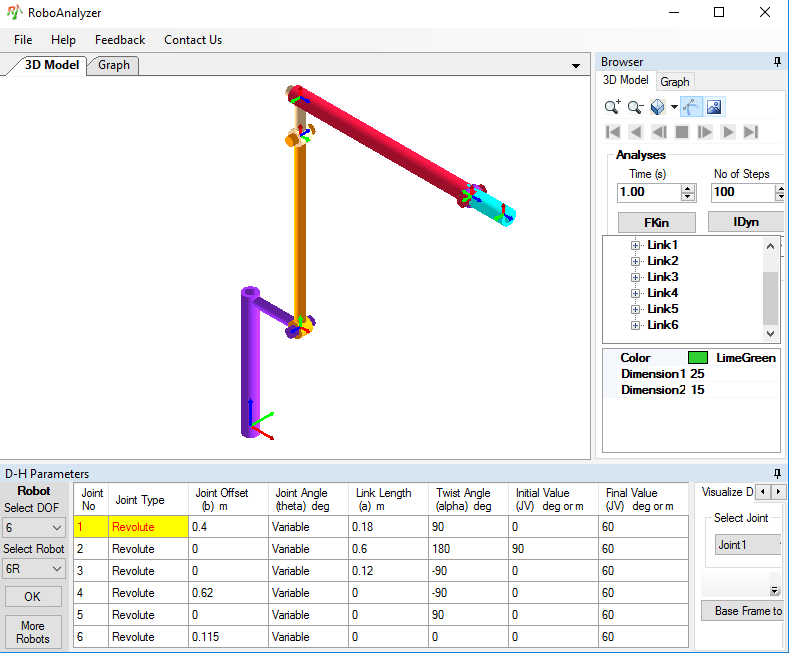
\includegraphics[width=0.95\textwidth]{pic_dh_kuka}
\caption{Vizualizace DH parametrizace robota KUKA KR5 Arc.}
\label{dh_kuka_pic}
\end{figure}

